
\section{Equilibrium}
 A board has reached quilibrium after $g$ generations if, in the $g+1$-th generation, no one has moved.\\
One of the research questions was: will the board reach an equilibrium (that is, no more moves)? Based on intuition, this is expected to be true. An individual who moves, does this to a place where there are relatively more neighbours of her type, so most of the time there are more individuals that gain happiness than those who lose happiness. In the basic model however, this is almost always true, but sometimes we get a periodic solution:\\
\begin{figure}[H]
	
    \centering
    \begin{subfigure}{0.3\textwidth}
        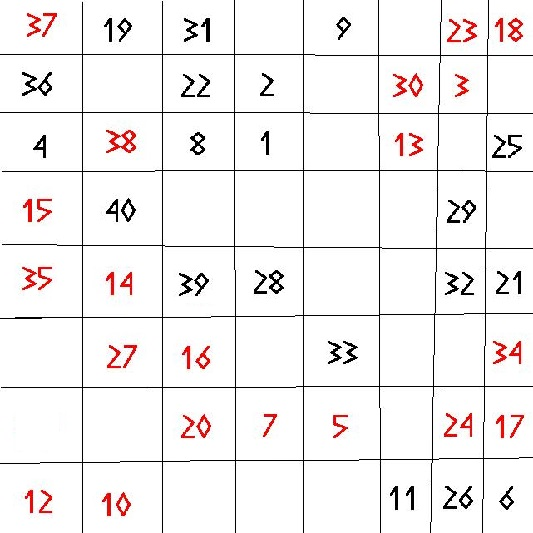
\includegraphics[width=\textwidth]{Tegenvoorbeeld/segregation_tegenvb.jpg}
        \caption{The start situation. Individual 37 is on her turn.}
        \label{fig:movement1}
    \end{subfigure}\hspace{1cm}
    ~ %add desired spacing between images, e. g. ~, \quad, \qquad, \hfill etc. 
      %(or a blank line to force the subfigure onto a new line)
    \begin{subfigure}{0.3\textwidth}
        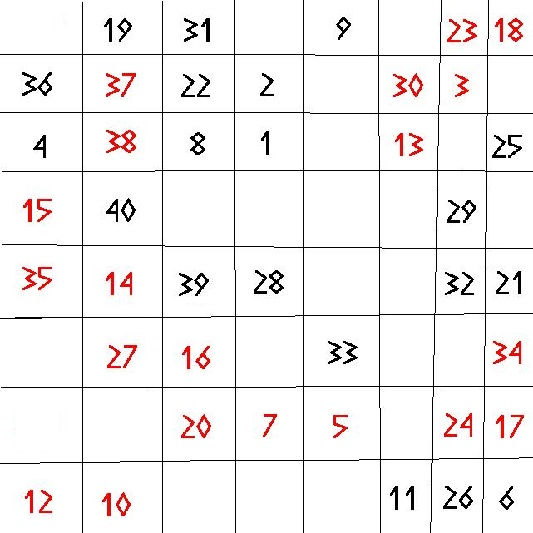
\includegraphics[width=\textwidth]{Tegenvoorbeeld/segregation_tegenvb_1.jpg}
        \caption{Individual 37 is moved to the nearest place that better meets her desire. }
        \label{fig:movement2}
    \end{subfigure}
    ~ %add desired spacing between images, e. g. ~, \quad, \qquad, \hfill etc. 
    %(or a blank line to force the subfigure onto a new line)
    \begin{subfigure}{0.3\textwidth}
        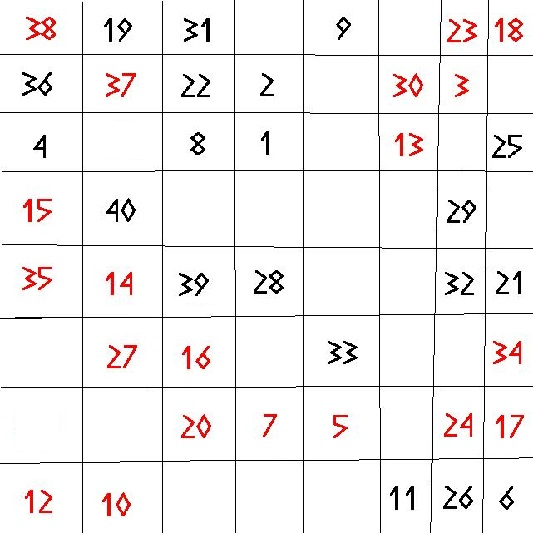
\includegraphics[width=\textwidth]{Tegenvoorbeeld/segregation_tegenvb_2.jpg}
        \caption{Individual 38 is on her turn and is moved to the nearest place that better meets her desire.}
        \label{fig:movement3}
    \end{subfigure}\hspace{1cm}
    \begin{subfigure}{0.3\textwidth}
        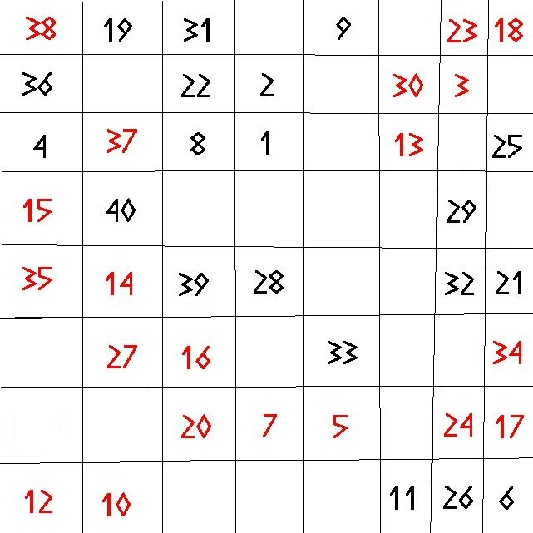
\includegraphics[width=\textwidth]{Tegenvoorbeeld/segregation_tegenvb_3.jpg}
        
        \caption{A generation has passed, 37 is on her turn and is moved to the nearest place for higher happiness. Because 37 and 38 are of the same type, this process repeats. }
        \label{fig:movement4}
    \end{subfigure}
    \caption{A possible configuration of the standard board in which the equilibrium will not be reached. The numbers indicate the selecting order of an individual. The two different colour indicates the two types. The equilibrium is not reached due to the periodic movements of individuals 37 and 38. The movements of inviduals 37 and 38 are tracked and shown in subfigure a to d in a chronological order.}\label{fig:equilibrium counterexample}
\end{figure}
In figure 2, a possible configuration in which the equilibrium will not be reached is shown. The numbers stand for the turn order (1 is selected first, then 2, etc.). Red and black stand for the 2 types. After some checkwork, we see that individuals 1 to 36 are all happy, but 37 is not. In 37's turn, we see that 37 has a happiness of $0$, and the closest empty spot has happiness of $\frac{1}{7} > 0$, so 37 will move to that spot, which is indicated in figure 1b.
\\Next, it's 38's turn. 38 has a happiness of $\frac{2}{7}$, which is less than the required $\frac{1}{3}$. The closest spot with greater happiness is the nearby corner spot with happiness $\frac{1}{3}$. So 38 will now move to the place which is shown in figure 2c.\\
The others will remain happy and will not move. When it's 37's turn again, 37 has happiness $\frac{1}{7} < \frac{1}{3}$. The closest empty spot has happiness $\frac{1}{6} > \frac{1}{7}$, so 37 will move to that spot. Now 37 and 38 have swapped position, as it is shown in figure 2d.\\
Since 37 and 38 are of the same type, those 3 moves will repeat: we have a periodic solution.\\
\textbf{Now what went wrong?} After the first move, both 37 and 38 will gain happiness, but on the third move, 38 will lose all of her happiness. We get an endless loop.\\
Note that, for larger boards, this periodic solution can still appear, because we can keep the individuals near the periodic solution the same, or even put everything in the upper left corner.
